Serial Parrallel Interface (SPI) er en måde at lave hurtig seriel dataudveksling på. SPI er udviklet af Motorola og fungerer ved at man, som regel, har en enkelt masterenhed der styrer flere slaveenheder. Ved SPI er der er ingen fejl-check og adressering af flere enheder kan være HW krævende. I EasyWater8000 projektet er der SPI kommunikation imellem Master (Devkit8000)
og Enhed (PSoC4), det giver muligheden for at overføre flere data på samme tid imellem disse to.

\begin{figure}[H] \centering
{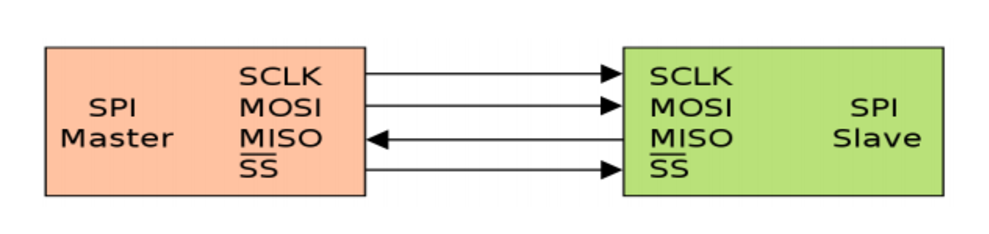
\includegraphics[width=\textwidth]{filer/design/Billeder/SPI_MASTER_SLAVE}}
\caption{Typisk opsætning af forbindelser imellem to enheder med SPI-kommunikation}
\label{lab:SPI}
\raggedright
\end{figure}

På figur \ref{lab:SPI} ses en typisk opkobling imellem Master og Slave, det kræver 4 tråde.
\begin{itemize}
 	\item SS står for "Slave select".
 	\item MISO står for "Master in slave out".
 	\item MOSI står for "Master out slave in". 
	\item SCLK står for "Serial clock" 
\end{itemize}

SPI-kommunikation er baseret på skifteregisterprincippet, som ses på figur \ref{lab:SPI_REGISTER}. Der vælges hvilken slave der 
ønskes at skrives til ved slave select(SS), derefter shiftes et 8-bit register 1 bit ad gangen. Serial clock er den clock der sørger for at
shiftningen af bits sker korrekt, clockfrekvensen må ikke overstige grænsen for hvad enhederne kan håndtere.

\begin{figure}[H] \centering
{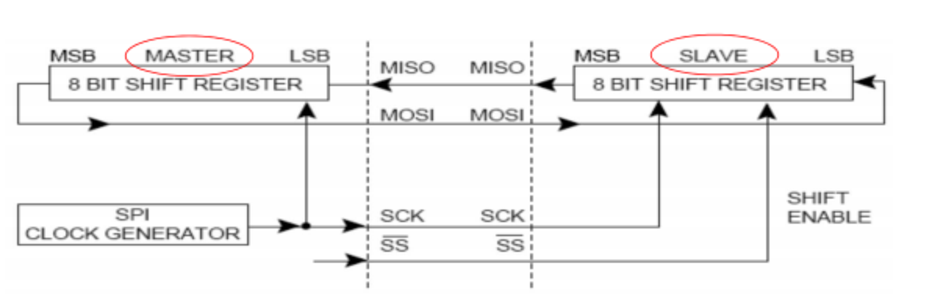
\includegraphics[width=\textwidth]{filer/design/Billeder/SPI_REGISTER}}
\caption{Beskrivelse af hvordan data flyttes igennem registre imellem Master og Slave med SPI-kommunikation}
\label{lab:SPI_REGISTER}
\raggedright
\end{figure}  

En ofte anvendt kommunikation imellem master og slave foregår ved at master sætter SS til 0. Den fortæller nu til slaven at den er klar til 
dataoverførsel. Nu sender masteren en bit over til slaven og påbegynder en half-duplex data transmission, samtidigt sender slaven en bit over til masteren. Denne process fortsætter indtil masteren har sendt alle sine bits, derefter stopper masteren med at toggle på clocken og slave enheder bliver frigivet.

SPI kan køre både full- og halfduplex, dvs. at der kan være 2-vejs kommunikation ved full-duplex (flere masterenheder) eller 2-vejs kommunikation ved half-duplex, hvor en masterenhed styrer/skriver til en eller flere slaveenheder. I EasyWater8000 er der behov for at der kommunikeres 2 veje, men da Enheden fungerer som slave, kan den ikke selvstændigt sende til Masteren, men behøver et kald, om at nu skal den sende information. Derfor er det half-duplex der bruges.